\section{Nintendo}
Nintendo is a Japanese multinational consumer electronics and video game company
headquartered in Kyoto, Japan. Nintendo is one of the world's largest video
game companies by market capitalization. Founded on 23 September 1889
by Fusajiro Yamauchi\cite{Nintendo}.\\

Nintendo is one of the 6 main consoles analized in this report; it has 10
platforms (mobile and house-only). and is one of the most known
video game consoles. Each platform has several games and has one
\textit{iconic} game that has the most sales, the platforms discussed with
their respective games are:\\

\subsection{Nintendo Entertainment System (NES):} The platform is an 8-bit
console initially released in Japan as the Family Computer in 1983, 1985 in
US and between 1986-1987 in Europe.\cite{Nintendo}. According to the data,
there are registered 98 games for this platform; for a total sales of \$251.07
million dollars. The most significant games are \textit{Mario Bros, Duck Hunt} and
\textit{Mario 3}.\\
\subsection{Super Nintendo (SNES):} This was a 16-bit video game console,
which was released in North America in 1991, and in Europe in 1992. The
console was initially released in Japan in 1990\cite{Nintendo}. The most
representative game for this platform is \textit{Super Mario World}, released in 1990
with total sales of \$20.61 million dollars.\\
\subsection{Gameboy:} Released in Japan on 21 April 1989, and in
North America on 31 July 1989\cite{Nintendo}. It got a total sales of 255.45
million dollars with 98 games released in total. The most representative games
for this platform where \textit{PokemonRed/Blue} with a total sales of 31.37 million
dollars, \textit{Tetris} (1989) with a total sales of \$30.26 million dollars and \textit{pokemon
gold / silver} with \$23.1million dollars in 1999.\\
\subsection{Nintendo 64:} Released in 1996, it featured 3D polygon model
rendering capabilities and built-in multiplayer for up to four
players\cite{Nintendo}. This platform accounted \$218.88 million dollars in
total sales spread in 319 released games. Its most representative game is
\textit{Mario 64}, published by Nintendo itself with total sales of \$11.89 million
dollars.\\
\subsection{Gameboy Advance:} Introduced in 2001 as a redesigned version of
the Gameboy\cite{Nintendo}. The most representative game for this platform is
\textit{Pokemon Ruby / Saphire}, with a total sales of \$15.85 million dollars
in 2002.\\
With 822 games released for this platform; the total sales where just 24\%
more than the Gameboy according to the data for \$318.5 million dollars in
total sales.\\
\subsection{GameCube:} released in 2001, in Japan and North America, and in
2002 worldwide. Its the successor of the Nintendo 64 and competed with Sony's
PlayStation2, Miscrosoft's Xbox and SEGA's Dreamcast\cite{Nintendo}. The
GameCube managed to get a total sales of \$199.36 million dollars with 556
games. Sales wise it did worse than its predeccessor the Nintendo 64. The 3
most representative games sales wise are \textit{Super Smash Bros Melee} (2001) with a
total sales of \$7.07 million dollars, \textit{Mario Kart: Double Dash} (2003) with \$6.95
million dollars in total sales and \textit{Super Mario Sunshine} with \$6.31 million
dollars in 2002.\\
\subsection{Nintendo DS:} In 2004, Nintendo released the Nintendo DS, its
fourth major handheld system. The DS is a dual screened handheld featuring
touch screen capabilities\cite{Nintendo}. These novel features account for
the great total grand sales of \$807.1 million dollars from 2152 released
games. Its the platform under Nintendo with the most games released. The most
representative game is \textit{New Super Mario Bros} which got released in 2006
accounting for sales of \$29.8 million dollars. Other relevant games are
Mario Kart DS with \$23.21 million dollars in sales and \textit{Nintendogs} with \$24.67
million dollars in sales.\\
\subsection{Nintendo 3DS:} This platform was an attempt to further expand the
Nintendo DS line, the Nintendo 3DS uses the process of autostereoscopy to
produce a stereoscopic three-dimensional effect without glasses. The 3DS got
off to a slow start, initially missing many key features but price cuts and
game releases helped to boost the 3DS sales. In August 2013, the 3DS was the
best selling console in the United States for four consecutive
months. The total sales of this platform was \$259.1 Million dollars;
Representative games for this platform are \textit{Pokemon X/Y} (2013) with
\$14.6 million dollars in sales and \textit{Mario Kart 7} in 2011 with
\$12.66 million dollars.\\
\subsection{Nintendo Wii:} The Wii was released during the holiday season of
2006 worldwide. The system features the Wii Remote controller, which can be
used as a handheld pointing device and which detects movement in three
dimensions. Another notable feature of the console is WiiConnect24, which
enables it to receive messages and updates over the Internet while in standby
mode. It also features a game download service, called "Virtual Console",
which features emulated games from past system.\cite{Nintendo}. This is the
console from Nintendo that has the most sales; it sold in total \$908.13
million dollars with 1320 games that belong to this platform. \textit{Wii Sports} is
the most prominent game with \$82.53 million in sales followed by \textit{Mario
  Kart wii} with \$35.52 million.\\
\subsection{Nintendo Wii U:} The Wii U is the successor to the Wii, it was
released during the holiday season of 2012 worldwide. The Wii U is
the first Nintendo console to support high-definition graphics. The Wii U's
primary controller is the Wii U GamePad, which features an embedded
touchscreen. The system supports most Wii controllers and
accessories\cite{Nintendo}. In contrast with the Wii; the Wii U was a total
failure. Up until 2016 it has 147 games and only sold \$82.16 million dollars.\newpage

In conclusion the best selling platform Nintendo has had is the Wii with a
total of \$908 million dollars in sales followed by the Nintendo DS with \$807
million dollars. The most relevant game across the whole nintendo Brand is
Mario and sometimes is has the game that sells the most in its platform. For
more info on all the games each platform has, point \textit{ARMeet} to
Figure\ref{fig:NintendoImage} to see each platform detailed sales.\\

%% on Figure~\ref{fig:OrganizationChart} Left.

\begin{figure}[h]
  \centering
  \centerline{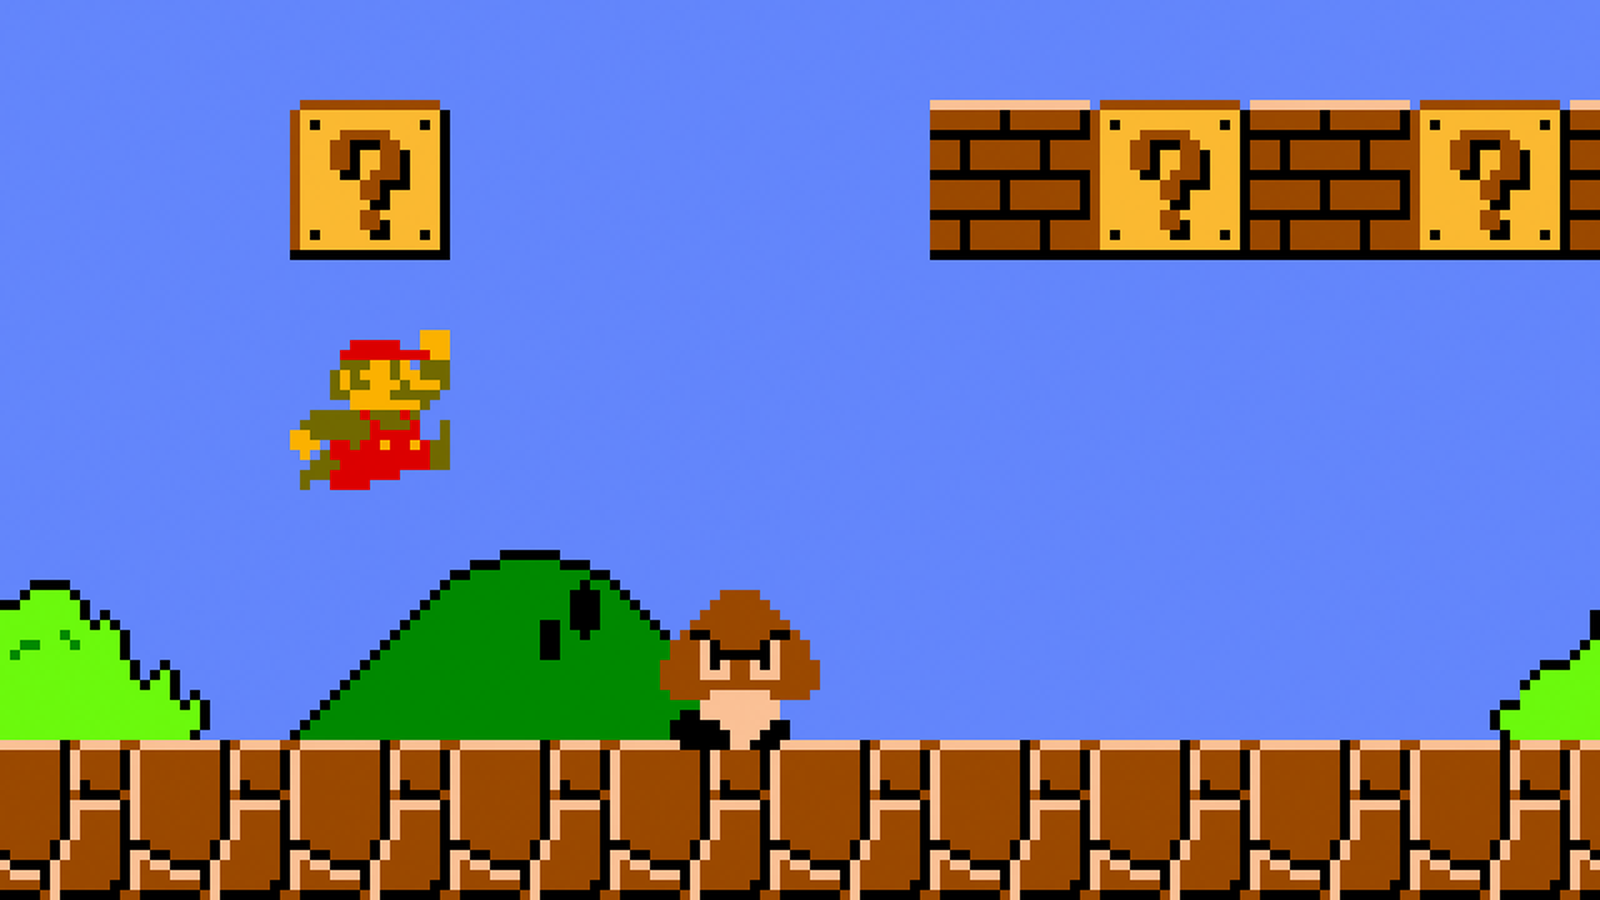
\includegraphics[scale=0.3]{images/NintendoMainTarget.png}}
  \caption{Representative picture of Nintendo, point ARMeet to this image to
    see the different sales on each platform.}
  \label{fig:NintendoImage}
\end{figure}


%% Platform: NES Games: 98
%% Total Sales: 251.07, by country US: 125.94 EU: 21.15 JP: 98.64999 Other: 5.310004
%% Platform: SNES Games: 239
%% Total Sales: 200.05, by country US: 61.22999 EU: 19.04 JP: 116.55 Other: 3.219999
%% Platform: GB Games: 98
%% Total Sales: 255.45, by country US: 114.32 EU: 47.82 JP: 85.12 Other: 8.200003
%% Platform: GBA Games: 822
%% Total Sales: 318.4997, by country US: 187.5397 EU: 75.25011 JP: 47.33 Other: 7.730047
%% Platform: N64 Games: 319
%% Total Sales: 218.8799, by country US: 139.02 EU: 41.05999 JP: 34.22 Other: 4.379999
%% Platform: GAME_CUBE Games: 556
%% Total Sales: 199.36, by country US: 133.4597 EU: 38.70978 JP: 21.58001 Other: 5.180024
%% Platform: DS Games: 2152
%% Total Sales: 807.1047, by country US: 382.6687 EU: 188.8892 JP: 175.57 Other: 59.27914
%% Platform: N3DS Games: 520
%% Total Sales: 259.0905, by country US: 83.49001 EU: 61.47997 JP: 100.67 Other: 13.36004
%% Platform: WII Games: 1320
%% Total Sales: 908.1315, by country US: 496.8999 EU: 262.21 JP: 69.32998 Other: 79.07024
%% Platform: WIIU Games: 147
%% Total Sales: 82.15997, by country US: 38.09999 EU: 25.13001 JP: 13.01 Other: 5.950011
